%
% File: chap01.tex
% Author: Victor F. Brena-Medina
% Description: Introduction chapter where the biology goes.
%
\let\textcircled=\pgftextcircled
\chapter*{Introduction}
\label{chap:intro}
\addstarredchapter{Introduction}
\markboth{Introduction}{}
\section*{CONTEXT}
\initial{S}erver virtualization allows the multiplexing of hardware resources on a physical computer for virtual machines\footnote{A virtual machine is the billing unit in the cloud. One consumes virtual machines possessing computing resources} (VM) that can then be purchased by companies in order to achieve power saving costs, machine acquirement savings, avoid licensing costs and servers maintenance. The server virtualization market is gaining demand as organizations seek to improve their business growth by shifting from on-premise to cloud based. Cloud providers such as Amazon, Microsoft, IBM, Google must ensure the isolation of virtual machines between them and make sure that a virtual machine possesses the resources for which a customer paid for the \acrshort{sla} to be met. To achieve this, they use server virtualization systems commonly known as hypervisors or virtual machine monitors (VMMs). Several hypervisors exist but our work relies on the Xen virtualization system firstly due to its \glspl{ops} nature, secondly because it is the hypervisor used by the Amazon Web Service \citep{aws-ec2}, who is the world leader cloud infrastructure provider \citep{aws-leader}. 

\par Xen is a server virtualization system that replaces the traditional operating system and runs directly on the hardware. It runs virtual machines in environments known as \textbf{domains}, which encapsulate a complete running virtual environment \citep{xen_book}. For the sake of simplicity and maintainability, the original operating system is embedded in a particular domain called \textbf{dom0} which stands for \textbf{domain 0} (the other domains are called \textbf{domU} meaning \textbf{domain unpriviledged}). The dom0 embeds administration tools for managing virtual machines (monitoring and configuration) in the overall \glspl{dc}. The most obvious task performed by the dom0 is to handle devices on behalf of the domU guests. It  includes \textbf{\glspl{dd}s} which provide access to the hardware as shown on Figure \ref{fig:arch_simple_xen}. The dom0 is therefore granted privileged access rights and can be seen as an extension of the hypervisor.

\begin{figure}[!h]
	\centering
    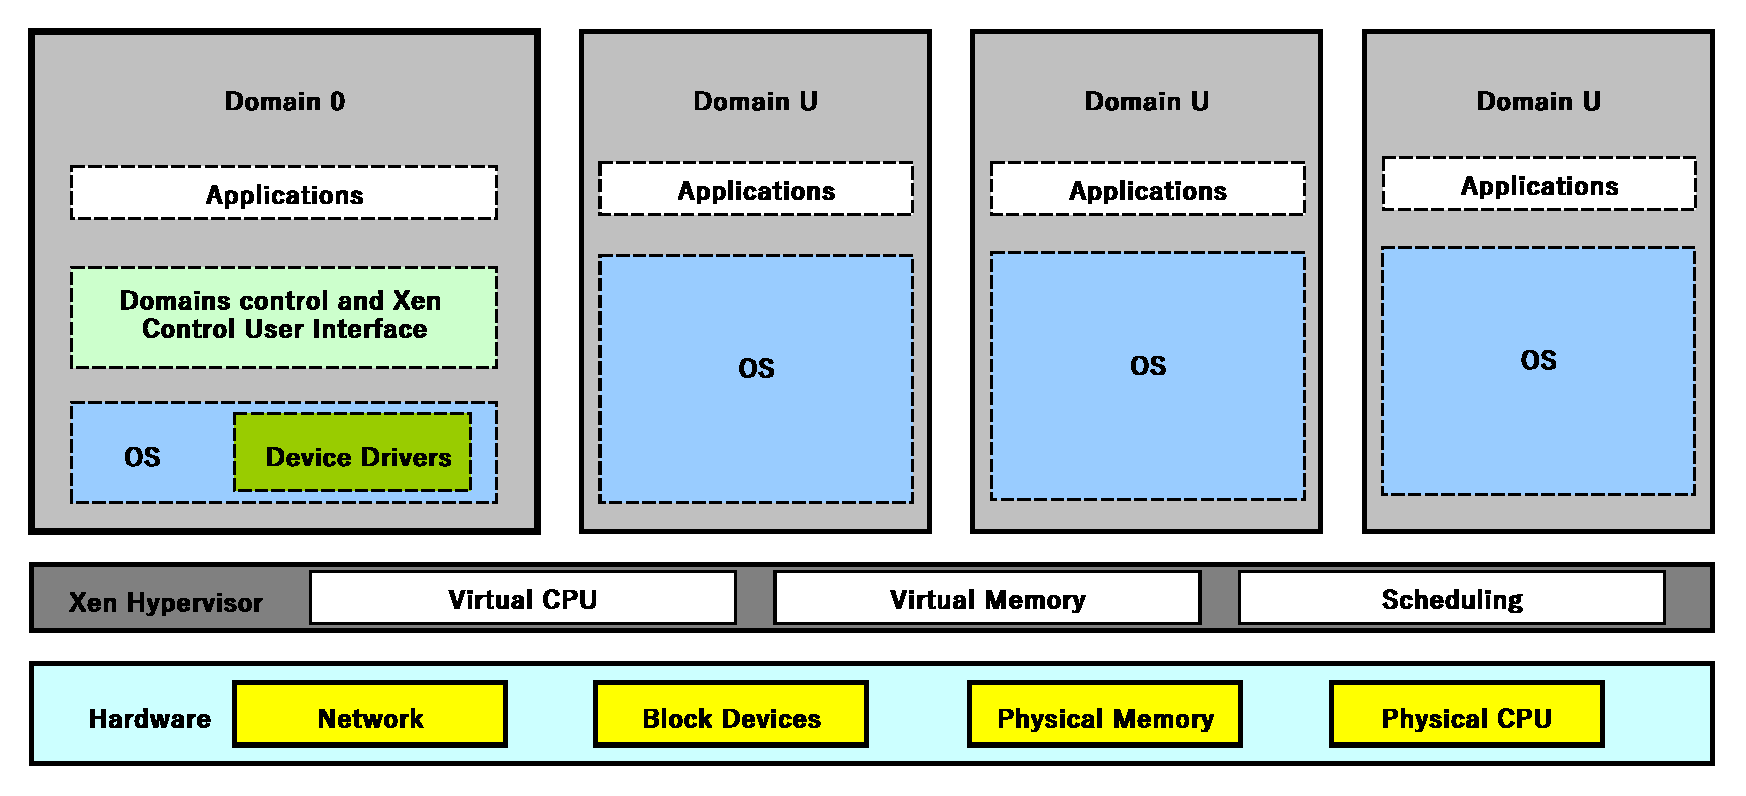
\includegraphics[width=\linewidth]{fig01/xen_simple.pdf}
    \caption{Simplified Xen Architecture}
    \label{fig:arch_simple_xen}
\end{figure}

\section*{PROBLEMATIC}

In order to perform all these tasks, the dom0 requires computing resources. As computing resources, we refer to \acrshort{cpu} and memory since the other resources such as network and disk are not significantly involved in these tasks. Resource allocation to the dom0 is a serious problem, especially in \acrshort{numa} architectures which are commonly used in today's \glspl{dc}s \citep{numa-most}. Concretely, cloud providers are faced with this essential question: 

\begin{bidentidad}{Question}
\begin{itemize}
    \centering How should resources be allocated to the dom0 and organised in a \\ \acrshort{numa} architecture ? 
\end{itemize}
\end{bidentidad}

\section*{OBJECTIVES}
The main goal of this work is to establish a \textbf{resource allocation strategy for the dom0} that will take into consideration the two fundamental questions mentioned above. Our resource allocation strategy should enable: 

\begin{enumerate}
    \item the dom0 to have exactly the amount of resources it needs at every moment,
    \item the dom0 processes that work on behalf of a virtual machine use the resources of this virtual machine and 
    \item those processes must be executed as close as possible to the virtual machine for which they work.
\end{enumerate}

To achieve this, we explored the issues associated with these two questions, analyzed the limitation of previous solutions addressed to this problem and compared our resulting model to the existing solutions on a series of \glspl{bench}s well thought out for the problem.

\section*{ROAD MAP}
The rest of the document is structured as follows: 

\begin{itemize}
    \item \textbf{Background} in which we enrich our vocabulary and present some mechanisms in the Xen architecture for a better understanding of the work and what follows;
    \item \textbf{Problem statement and assessment} where we discuss about the questions raised in the problematic and prove it is relevant;
    \item \textbf{Contribution} in which we describe our model, with a view on the overall architecture and a detailed presentation of the different model components;
    \item \textbf{Implementation and Evaluation} where we describe how our model has been developed, the different software tools used and how our solution performs compared to the existing solutions in order to verify if our solution meets the objectives defined.
\end{itemize} 
